%		DOCUMENT CLASS			%
\documentclass[conference]{IEEEtran}

%		PACKAGES & MACROS		%
\usepackage{graphics}
\usepackage{epsfig}
\usepackage{mathptmx}
\usepackage{amsmath}
\usepackage{amssymb} 
\usepackage{listings}
\usepackage{color}
\usepackage{url}
\usepackage{graphicx}
\usepackage{subfig}
\usepackage{caption}
\usepackage{algorithmic}
\usepackage{algorithm2e}

% commands
\renewcommand{\Re}{{\mathbb{R}}}
\newcommand{\R}{{\mathbb{R}}}
\newcommand{\Q}{{\mathbb{Q}}}
\newcommand{\Ze}{{\mathbb Z}}
\newcommand{\B}{{\mathbb B}}
\newcommand{\Ce}{{\mathbb C}}
\newcommand{\N}{{\mathbb{N}}}
\newcommand{\T}{{\mathbb T}}
\newcommand{\ie}{{\it i.e.}}
\newcommand{\eg}{{\it e.g.}}
\newcommand{\ea}{{\it et al }}
\renewcommand{\r}{\textcolor{red}}
\renewcommand{\b}{\textcolor{blue}}
\newcommand{\bk}{\textcolor{black}}
\newcommand{\argmin}{\textrm{arg}\min}
\newcommand{\Pre}{\mathrm{Pre}}
\def\transform{{\mathsf{filter}}}
\def\xduce{{\mathsf{xduce}}}
\def\set#1{{\{ #1 \}}}

%	HYPHENATION CORRECTION	%
\hyphenation{}

%		BEGIN DOCUMENT			%
\begin{document}

%		    PAPER TITLE    			%
\title{VaRTOS: Optimizing Application Utility with Variable Hardware }



%		AUTHOR NAMES			%
% author names and affiliations
% use a multiple column layout for up to three different
% affiliations
\author{
\IEEEauthorblockN{Paul Martin$^\dagger$, Lucas Wanner$^*$, Puneet Gupta$^\dagger$, \& Mani  Srivastava$^\dagger$}
\IEEEauthorblockA{$^\dagger$Department of Electrical Engineering, $^*$Department of Computer Science\\
University of California, Los Angeles\\
Email: \{ pdmartin, wanner, mbs \} @ucla.edu ~~ \{ puneet \} @ee.ucla.edu }\\
\vspace{5mm}
}


% make the title area
\maketitle


%			ABSTRACT			%
\begin{abstract}

Increasing hardware variability in newer fabrication technologies has spurred research in kind, spanning the entire spectrum of computing.  One domain that stands to benefit greatly from research into combatting hardware variation is that of low power embedded systems and low power sensors. Systems tasked with performing sensing, routing, and inference tasks over extended lifetimes with limited energy reserves often resort to very liberal duty cycling, reducing the total active time spent on any given task.  The lifetimes of such systems are largely dominated by leakage power in idle states---an entity that is greatly affected by hardware variation. We present VaRTOS, an architecture and corresponding kernel extensions that provide explicit treatment of both sleep and active power variations for duty cycled tasks running in real time operating systems. VaRTOS seeks to maximize application utility while converging on an optimal duty cycle both on a per-task basis and on a system-wide basis.  In doing so, we provide results regarding online learning of instance-specific sleep power, active power, and temperature profiles on simulated hardware with demonstrated effects for several prototypical applications. 

\end{abstract}

\IEEEpeerreviewmaketitle


%		INCLUDED SECTIONS		%
\section{Introduction}
\label{sec:introduction}

The emergence of low power wireless systems in past decades was followed by attempts at optimizing energy efficiency and power consumption to facilitate long lifetime sensing deployments.  
%Research in this area was marked by many successes in the form of efficient time synchronization algorithms, routing protocols, new sensing paradigms, and the emergence of several widely-adopted operating systems for embedded systems (e.g., [\citeNP{tinyos}; \citeNP{contiki}]).
 In recent years, newer integrated circuit fabrication technologies have introduced several additional variables into the energy management game; as feature sizes continue to shrink, power variation on a per-instance level has become a non-trivial factor [\citeNP{Borkar:2003}; \citeNP{gupta2003}]. 

%Figure \ref{fig:variation} offers more intuition into the matter, showing the projected variation in idle and overall power as projected by the International Technology Roadmap for Semiconductors (ITRS) for years to come \cite{ITRS} as well as recent variability results in the literature. 

%\begin{figure}
%\centering
%\includegraphics[width=0.5\textwidth]{figures/projected_variations}
%\caption{\label{fig:variation}ITRS projections for sleep and idle power variability with measurements from recent %literature.}
%\end{figure}

Per-instance power variations are particularly exaggerated for idle power consumption, motivating the need to mitigate the effects of variability in systems whose operation is dominated by long idle states.  Figure \ref{fig:itrs} provides more insight into the matter: the International Technology Roadmap for Semiconductors (ITRS) predicts as much as 600\% variation in static (idle) power and over 100\% in total power by the year 2022 \cite{ITRS}. One domain that stands to benefit from research into combatting hardware variation is that of low power embedded systems and low power sensors, where the application is often that of sensing, routing, or processing data.  

In systems where computation is severely constrained by anemic energy reserves and where a long overall system lifetime is desired, maximizing the utility of a given application subject to these constraints is both challenging and an important step towards achieving high quality deployments.  Currently, developers assume some power consumption model prior to deployment, and this can have several undesired effects.  Underestimation of system power consumption can lead to a reduction in lifetime which will eventually impact quality of service, while guardbanding against worst-case power consumption by using overly conservative estimates can reduce application quality for the entirety of the lifetime. The potential solution space is shown in Figure \ref{fig:qualityandlifetime}, where the optimal solution is one that maximizes quality without decreasing lifetime. Furthermore, the distribution of power in systems comprised of multiple heterogeneous tasks is oftentimes fixed in software prior to deployment as well, placing the burden of optimizing energy usage on developers who may remain oblivious to variations in power consumption altogether. 

%Considerable research has focused on exposing energy and power measurements or estimates to the developer and even to the end user.  For example, techniques using linear combinations of instruction and performance counters [\citeNP{sun2012}; \citeNP{singh2009}], activity monitoring strategies \cite{appscope}, and various battery discharge-based models \cite{zhang2010} have been explored as tools for providing system-wide, application-specific, and even per-process granularities of energy usage.  Improved techniques for accurately  estimating and measuring power consumption will enable online power management in ways that were infeasible before, helping mitigate fabrication-induced per-instance chip variation as well.

Perhaps the most widely used and most effective strategies for extending the lifetime of energy-constrained systems are those based on controlling the ratio of system active time to total system time, or \emph{duty cycling} a system.  Duty cycled systems take advantage of the disparity between active and idle power consumption, greatly increasing the lifetime of systems where latency and throughput constraints can be relaxed. Because of temperature and instance dependencies in power consumption, however, arriving at an optimal system-wide duty cycle ratio to achieve a lifetime goal given an energy constraint is difficult to do without \emph{a priori} knowledge of instance-specific power models and temperature statistics for the target deployment location \cite{Wanner:2012}. Furthermore, applications involving more than one task necessitate notions of fairness and utility---specifically, how should active processor time be distributed between each task so as to maximize the utility of the application and still meet the desired lifetime goal?

\begin{figure*}[t]
\centering
{\centering
\begin{minipage}{0.47\textwidth}
  \centering
\includegraphics[width=\textwidth]{figures/itrs}
  \captionof{figure}{\label{fig:itrs}ITRS predictions for processor power variation for years to come}
\end{minipage}
\hspace{.04\textwidth}
\begin{minipage}{0.47\textwidth}
  \centering
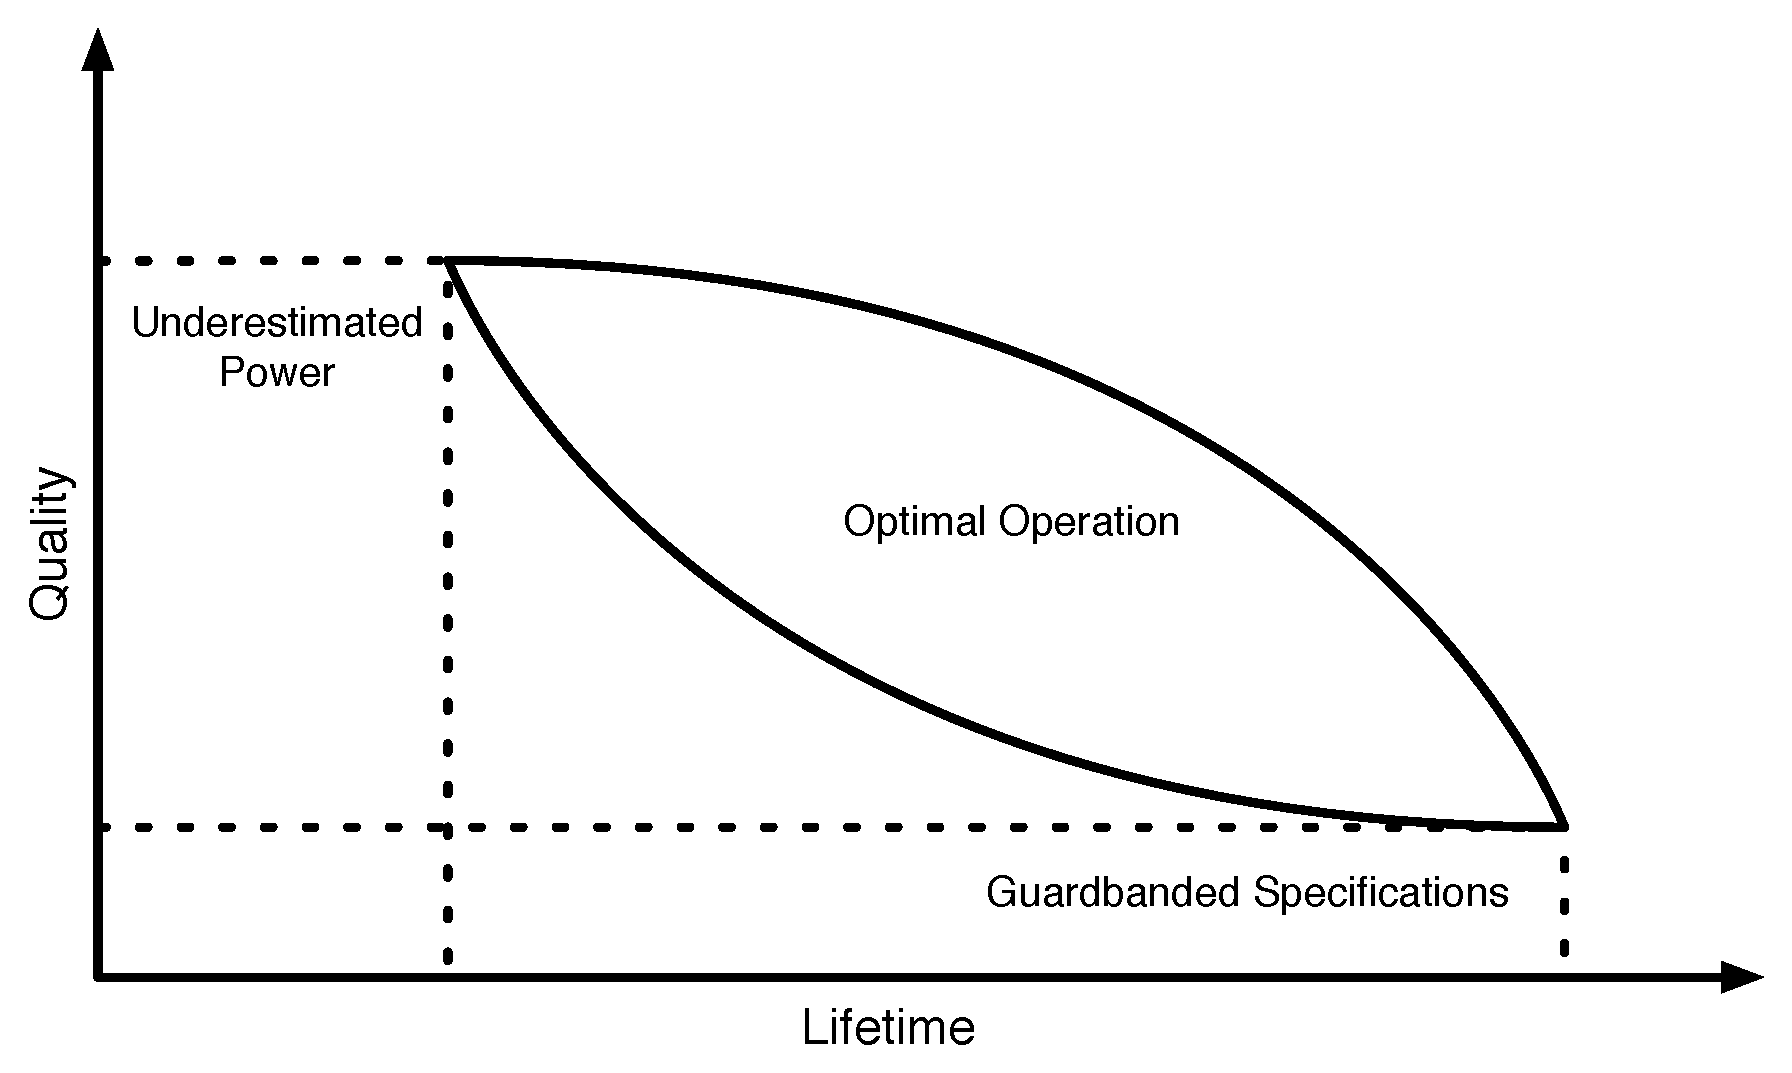
\includegraphics[width=\textwidth]{figures/intro_quality_vs_lifetime}
  \captionof{figure}{\label{fig:qualityandlifetime}potential results of variability in terms of system quality and lifetime}
\end{minipage}
}
\end{figure*}



In this work we explore the interplay between variable active and idle power consumption, deployment-specific temperature profiles, and multiple heterogeneous tasks. Specifically, we seek an answer to the question posed above; in an environment where power and temperature are measurable quantities, we seek an optimal strategy for distributing energy between arbitrary tasks in order to maximize application utility.  In answering these questions, we introduce the notion of task \emph{knobs}.  These knobs offer both a way for tasks to express elasticity in terms of utility and processing time and a way in which an operating system can fine-tune task energy consumption. Developers provide bounds on the values that each knob can assume and decide in what ways each knob is used, but optimization of these knob values is offloaded to the operating system and is done at runtime after accurate power and computational models have been constructed.  These operating system abstractions are implemented in VaRTOS, a variability-aware operating system built as an extension to an open-source embedded operating system. In order to evaluate the abstractions and architectures that make up VaRTOS, we use custom variability extensions to a popular hardware simulation suite. 

Our contributions include the following: 

\begin{itemize}
\item We develop an architecture for modeling and optimizing per-task energy consumption at the operating system level, allowing for tunable quality and, correspondingly, accurate lifetime achievement in the face of variability. 
\item We provide a tool for evaluating the effects of power variation, environmental temperature, and additional constraints on the quality of user-defined applications comprised of multiple tasks prior to system deployment.
\item We evaluate VaRTOS, a variability-aware embedded OS that requires a modest 6.8 kB of flash memory and 518 bytes of RAM
\item We evaluate the effects of VaRTOS on several prototypical case studies, using a modified version of the QEMU simulation suite \cite{qemu}.   Our results show that VaRTOS can reduce energy consumption error to below 2\% in most cases, while strategies that assume worst-case power consumption have $> 70\%$ error in many cases.
\end{itemize}



\section{Related Work}

Power management and longevity in wireless sensor networks and low power embedded systems in general has long been an active area of research.  Traditional power management techniques have assumed that, while idle and active powers vary as a function of temperature, they remain uniform across instances.  Of these variability-agnostic techniques, many have focused on the tradeoff between energy and utility or performance.  For example, \cite{green2010, ghasemzadeh2012} represent attempts at making quality energy-proportional and tunable.  Specifically, \cite{green2010} introduces an architecture that allows developers to specify multiple versions of functions whereby the operating system can sacrifice quality when possible to reduce computational costs.  Similarly, \cite{ghasemzadeh2012} proposes tunable feature selection for wearable embedded systems, where less accurate feature computation can be used at the cost of inference quality. Similarly, \cite{liu1994} represents one of many efforts at using approximate computing to save energy where marginal losses in quality can be afforded. 

More recent efforts have begun to consider hardware variability and methods for mitigating variation in software.  These can roughly be divided into two camps: (1) low-level treatment of variability in hardware and in voltage and frequency scaling (e.g. \cite{teodorescu2008}) and (2) application-level adaptations to meet power requirements.  While low-level treatment of hardware variation is undoubtedly a necessary step forward for commercial processors, application- and process-level adaptations have proven effective methods for combatting variation in low power embedded systems and wireless sensor networks.  Both \cite{matsuda2006} and \cite{garg2007} provide lifetime analyses for wireless sensor networks when considering variability power models, offering insights into what such systems stand to gain from explicit treatment of hardware variation.  Garg et al. estimated that a 37\% system lifetime improvement could be achieved through redundancy efforts that totaled a 20\% increased deployment cost.  To avoid cost increases, application quality or performance can be reduced as in \cite{pant2010}, where video compression codecs are selected based on particular hardware variability `signatures'.

This work is closely related to that of Wanner et al. in \cite{wanner2011}.  There, the authors describe a method for calculating a system-wide optimal duty cycle ratio given known models for active and idle power as well as probability density functions for deployment temperatures. Here we provide an extension to the work in \cite{wanner2011}, showing methods for online learning of power models and providing notions of utility in multi-task applications.  



\section{Power Variability}

As fabrication technologies improve and feature sizes decrease, hardware variation plays an increasingly important role in determine the power consumption and therefore lifetime of computer systems.  While the large baseline in active power consumption relative to idle power consumption amortizes these variations to some degree (\cite{wanner2011} cites a 10\% variation in active power while \cite{balaji2012} cites between 7\% and 17\% variation), the low baseline in idle power consumption renders it highly susceptible to fabrication-induced variations (\cite{wanner2011} reports a 14x range in measured idle powers across 10 instances of ARM Cortex M3 processors). 

Power consumption in energy-constrained embedded systems is often dominated by time spent in an idle state, waiting to sense, communicate, or perform a processing task. Consequently, the lifetimes of these systems can be wildly variant due to instance-to-instance variation in idle power.  The result of inaccurate lifetime estimates obtained by improper power models can be one of two things: conservative designs can make sure that lifetime is met by adding a guard band to system duty cycle and thus underperforming, or removing these guard bands will result in higher performance while all subsystems (perhaps nodes in a network) are still running, but upon depletion of energy reserves by those processors with higher power consumption the entire system will again suffer.  A processor-specific duty cycle can be assigned so that all lifetimes are met, but without a strategy for distributing resources to individual tasks on a processor there is no guarantee that these variations are handled elegantly and in a way that maximizes application utility.
\section{VaRTOS}
In this section we present VaRTOS---a variability-aware architecture and corresponding extensions to the FreeRTOS \r{cite here} kernel for optimizing application-wide utility.  In doing so, we will introduce models for heterogenous tasks that comprise an application as well as corresponding utility functions. 

\subsection{Task Modeling}
We start first by introducing an \emph{application} $A$ as a set of \emph{tasks} $\{T_1, T_2, \ldots, T_n \}$, where each task represents a periodic subprocess of $A$.  It is assumed that a task $T_i$ will add an increase in utility $\delta u_i$ when given additional active compute time, $\delta T_{a,i}$. Here, $u_i$ is a utility function specific to task $T_i$ and analogous to quality of service (QoS).  Whereas some efforts take the stance that the $u_i$ should be provided by the developer (\cite{green2010} for example), we advocate offloading the burden to the OS itself.  In doing so, we will assume that $u_i$ is a monotonically non-decreasing function of active computation time $T_a,i$ or, equivalently, the duty cycle ratio specific to $T_i$ denoted $d_i$.  Tasks will offer varying degrees of utility for different $d_i$, and so some degree of user input is required to guide the optimization routine in distributing active time in an efficient manner.  To incorporate this user input, we introduce the concept of a task \emph{knob}.

\noindent\textbf{Task Knobs}: 
In order to tune the active time used per task and thus the task-specific duty cycle ratio $d_i$, we introduce the notion of task knobs denoted $k_i$, with the intuition that increasing $k_i$ will increase $T_{i,a}$, $d_i$, and $u_i$.  In practical terms, a task knob is a variable that will govern either (1) the period of a task or (2) the frequency with which a task is activated. We argue that the vast majority of tasks found in embedded applications will fall in one of these two classes, and those that require both frequency and period modulation can often be divided into two legal subtasks glued together with inter-process communications. For example, those that fall in class 1 include variable length sensing tasks, listening for inbound communication, and variable length processing chains.  Those that fall in class 2 include variable frequency transmission, variable frequency sensor sampling, time synchronization handshaking, control and actuation events, and more.  

Task knobs are created by passing a variable pointer to the OS, allowing direct manipulation of knobs by the optimization routine.  In addition, the developer specifies a minimum and maximum knob value, $k_{i,min}$ and $k_{i,max}$. The value $k_{i,min}$ specifies the minimum amount of work $T_i$ must do in order for it to be useful. Below this value, a task offers no utility.  The value $k_{i,max}$ specifies a value at which increasing $k_i$ further will yield only marginal or no added utility.  As an example, a radio transmission task may be useless if it does not meet a certain latency requirement, but usefulness may plateau at some frequency governed perhaps by the physics and time response of the event being sensed. 

\noindent\textbf{Interpolating Utility}: given $k_{i,min}$ and $k_{i,max}$ we construct a utility function $u_i = f(d_i)$ as a logistic (Sigmoid) function of the form 

$$
u_i(d_i) = {1\over{1 + e^{-c_id_i}}}, ~~c_i \ge 0
$$

We require only the convex portion of the Sigmoid function, choosing $u_i(d_i)$ to be of the particular form

\begin{equation}
u_i(d_i) = { 2\over { 1 + e^{-c_id_i }} }- 1, ~~c_i \ge 0
\label{eq:util}
\end{equation}

Here, $c_i$ governs the convergence rate of $u_i$ from the minimum utility to the maximum utility and is calculated as a function of $k_{i,min}$ and $k_{i,max}$ such that 99\% of the utility has been reached by $k_{max}$.  Increasing the percentage of $u_{i,max}$ realized by $k_{i,max}$ has the effect of arbitrarily steepening the utility curve. The constant $c_i$ can then be calculated from Equation \ref{eq:util} as

\begin{equation}
c_i = { -log\left( {2\over \epsilon + 1} - 1 \right) \over d_{i,max} - d_{i,min} }, ~~\epsilon = 0.99
\label{eq:c}
\end{equation}

Finally, each utility curve can be arbitrarily scaled by a priority scalar $p_i$ for tasks with intrinsically higher utility than others. Figure \ref{fig:util} shows three example utility curves corresponding to three tasks with various priorities and duty cycle ranges (resulting from various $k_{i,min}$ and $k_{i,max}$). 

\begin{figure}
\centering
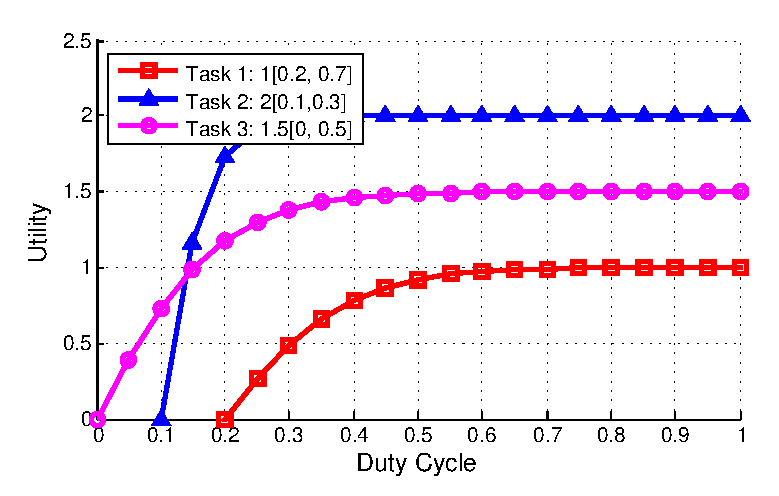
\includegraphics[width=1\columnwidth]{figures/utilityfunctions.eps}
\caption{\label{fig:util}Example utility curves. Task 1 has priority scalar 1 with useful range $d_i = [0.2, 0.7]$, task 2 with priority scalar 2 and so forth. }
\end{figure}

\noindent\textbf{Learning the $k_i \rightarrow T_{i,a}$ Relation}: Because the developer has free reign to use the knob $k_i$ for each task as desired, the function mapping $k_i$ to active time $T_{i,a}$ and thus $d_i$ is not known \emph{a priori}. Instead, the transformation $\mathcal{K}_i$ that maps $k_i$ to $T_{i,a}$  is assumed linear and is learned through regression at runtime. Should the developer misuse $k_i$ in a way that is nonlinear or results in non-increasing values of $T_{i,a}$, the optimization routine will suffer. Active time per task can be measured using hardware timer snapshots at the context swap level or other mechanisms described later in the text.  Given a method for measuring $T_{a,i}$, $\mathcal{K}_i$ is arrived at by systematic perturbation of $k_i$ within the range $[k_{i,min}, k_{i,max}]$. Specifically, $k_i$ is repeatedly increased by $\Delta = {k_{i,max} - k_{i,min} \over N}$ where $N$ is the number of points in the regression, kept sufficiently low ($N = 3$ in our case) to minimize memory footprint.  Between each perturbation in $k_i$, the task is allowed to run for a time period sufficiently long enough to capture active time measurements even for tasks with very infrequent activity.  In the applications presented here, this supervisory period is set at 1 hour. Dividing active time accumulated per task by the supervisory interval yields task-specific duty cycle ratios, $d_i$. 

\subsection{System-wide Duty Cycle}
Distributing active time per task assumes that we can afford a certain system-wide active time per supervisory interval, or equivalently that the system is governed by an optimal duty cycle $d^*$.  Arriving at $d^*$ is done in the same way as set forth in \cite{wanner2011} with the exception that the active and idle/sleep powers ($P_a$ and $P_s$) are learned at runtime.  The optimal duty cycle $d^*$ is calculated as a function of $P_a, P_s$, and $\pmb{f}_T$, where $\pmb{f}_T$ is the probability density function of the temperature for the location where the system is to be deployed. Given these quantities, $d^*$ can be found as a solution to the optimization problem

$$
d^* = \max ~~{d}~~\text{subject to:}
$$
\begin{equation}
\sum_Tf_T\left[dP_a(T) + (1-d)P_s(T)\right] \le {E\over L} = \bar{P}
\label{eq:opt}
\end{equation}

That is, maximize $d$ such that the lifetime and energy constraints are met.  Here, $E$ and $L$ are the energy and lifetime specifications and $\bar{P}$ is the average power needed to obtain lifetime $L$. The optimal solution to Equation \ref{eq:opt} can be obtained algebraically as shown in \cite{wanner2011}:

\begin{equation}
d^* =  { E - L\bar{P_s} \over L(\bar{P_a} -\bar{P_s}) } 
\end{equation}

Where $\bar{P_a}$ and $\bar{P_s}$ are temperature-averaged power quantities. 

\subsection{Optimizing Utility}
Because we have chosen $u_i$ to be a logistic function, we can use a greedy approach when optimizing utility.  The optimization routine will be a two step process: (1) attempt to assign the minimum duty cycle $d_{i,min} = \mathcal{K}_i(k_{i,min})$ needed for each task to yield utility in order of decreasing priority, and (2) continue distributing utility to the task 


\begin{figure}
\centering
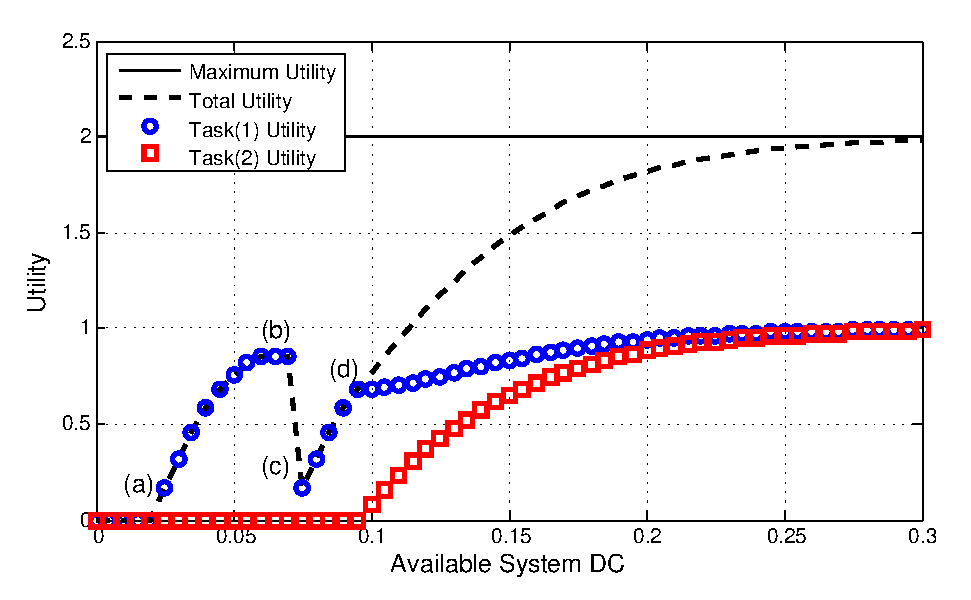
\includegraphics[width=1\columnwidth]{figures/optimalDCexample.eps}
\caption{\label{fig:optimaldc_mult}optimizing shit}
\end{figure}

\begin{figure}
\centering
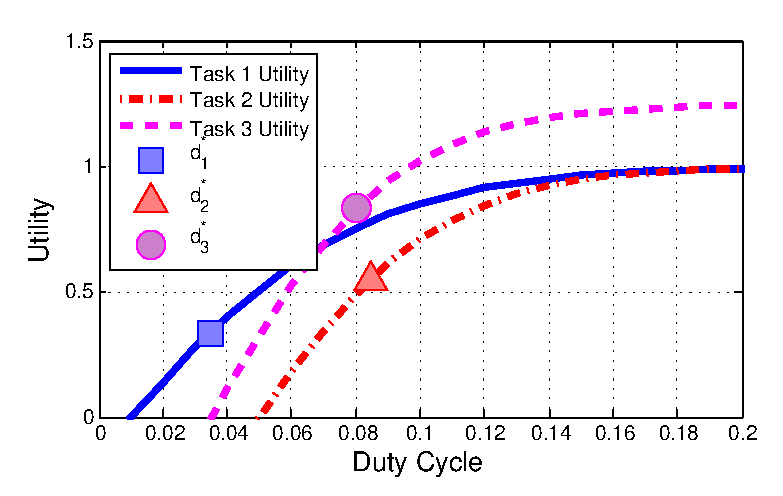
\includegraphics[width=1\columnwidth]{figures/utilanddc.eps}
\caption{\label{fig:utilanddc}optimizing shit}
\end{figure}

\begin{figure*}
\centering
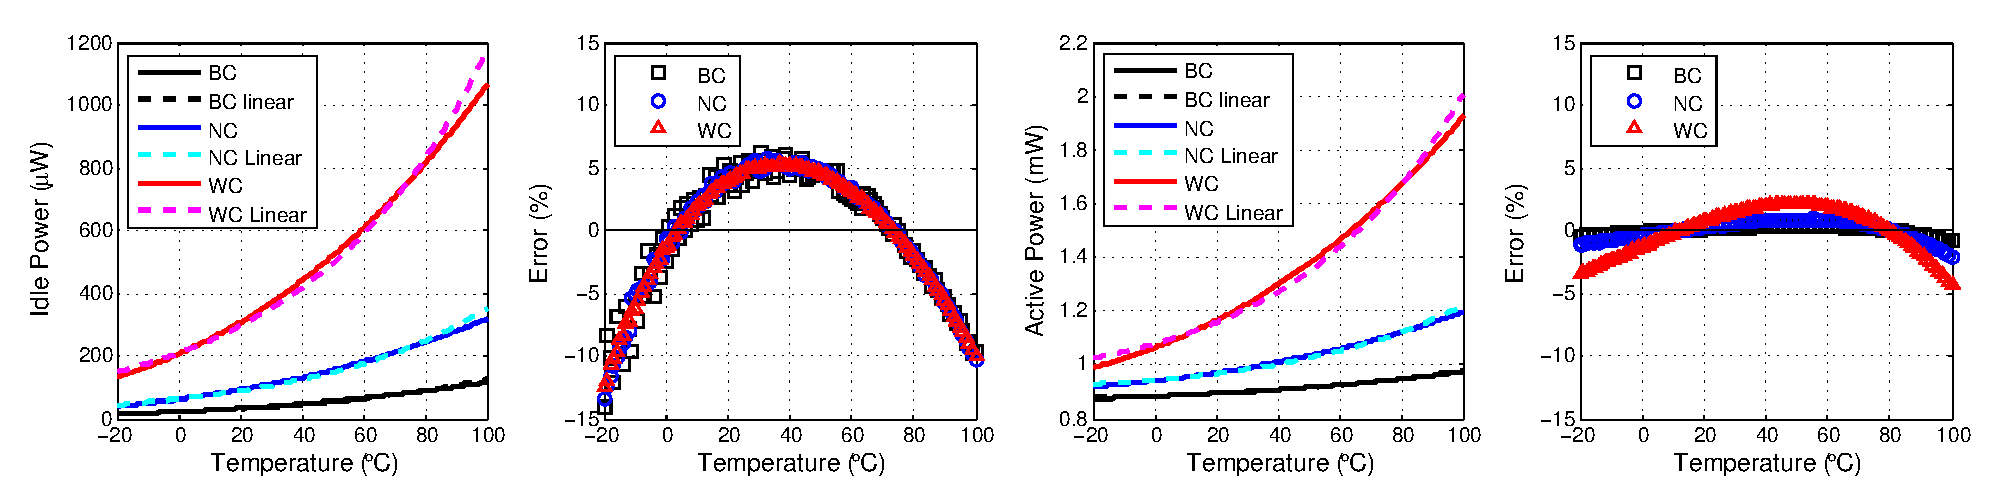
\includegraphics[width=1\textwidth]{figures/powerlearning.eps}
\caption{\label{fig:powerlearning}Learning power....}
\end{figure*}


%% Algorithm
\begin{algorithm}
 \SetAlgoLined
 \KwData{$u_a(d) \forall a \in A, ~d^*_T$}
 \KwResult{$d^*_a$ }
 $d_{remaining} \leftarrow d^*_T$.  \\
 Assign min knob values:\\
 \For{$a \in A$}{
 	\eIf{$d_a(k_{min}) < d_{remaining}$}{
 	$d_a = d_a(k_{min})$\\
	$d_{remaining} \leftarrow d_{remaining} - d_a$
 	}{
 	stop
 	}
 }
 Divvy up remaining duty cycle fairly:\\
 \While{$d_{remaining} > 0$}{
 	Find highest marginal utility:\\
	$maxM.U. \leftarrow 0$\\
	$numMax \leftarrow 1$\\
	 \For{$a \in A$}{
	 	\eIf{$m(a) > maxM.U.$}{
			$maxM.U. \leftarrow m(a)$
			$numMax \leftarrow 1$
		}{\If{$m(a) == maxM.U.$}{
			$numMax \leftarrow numMax + 1$
		}
		}
	 }
	 
	 Increment task duty cycles:\\
	 $d_{requested} \leftarrow \delta \cdot numMax$\\
	 \If{$d_{requested} > d_{remaining}$}{
	 	$d_{requested} \leftarrow d_{remaining}$
	 }
	 \For{$a \in A$}{
	 	\If{$m(a) == maxM.U.$}{
			$d_a \leftarrow d_a + d_{requested}/numMax$
		}
	 }
 }
 \caption{Greedy duty cycle optimization}
\end{algorithm}

\subsection{Instance Modeling}
including sleep and active power, and musings on learning the temperature profile etc.



\subsection{Operation}
Talk about what happens in steady state, how we check for errors, what happens when errors become large, etc. 

\begin{figure}
\centering
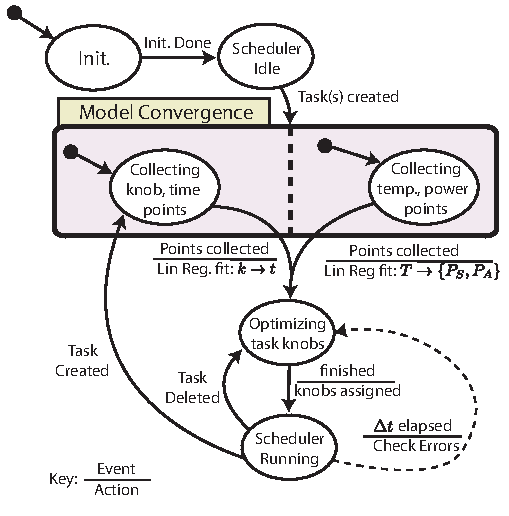
\includegraphics[width=1\columnwidth]{figures/statechart.pdf}
\caption{\label{fig:state chart}state chart}
\end{figure}

\begin{figure}
\centering
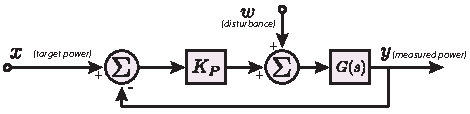
\includegraphics[width=1\columnwidth]{figures/controlloop.pdf}
\caption{\label{fig:state chart}state chart}
\end{figure}





\section{Evaluation}

\begin{figure*}
\centering
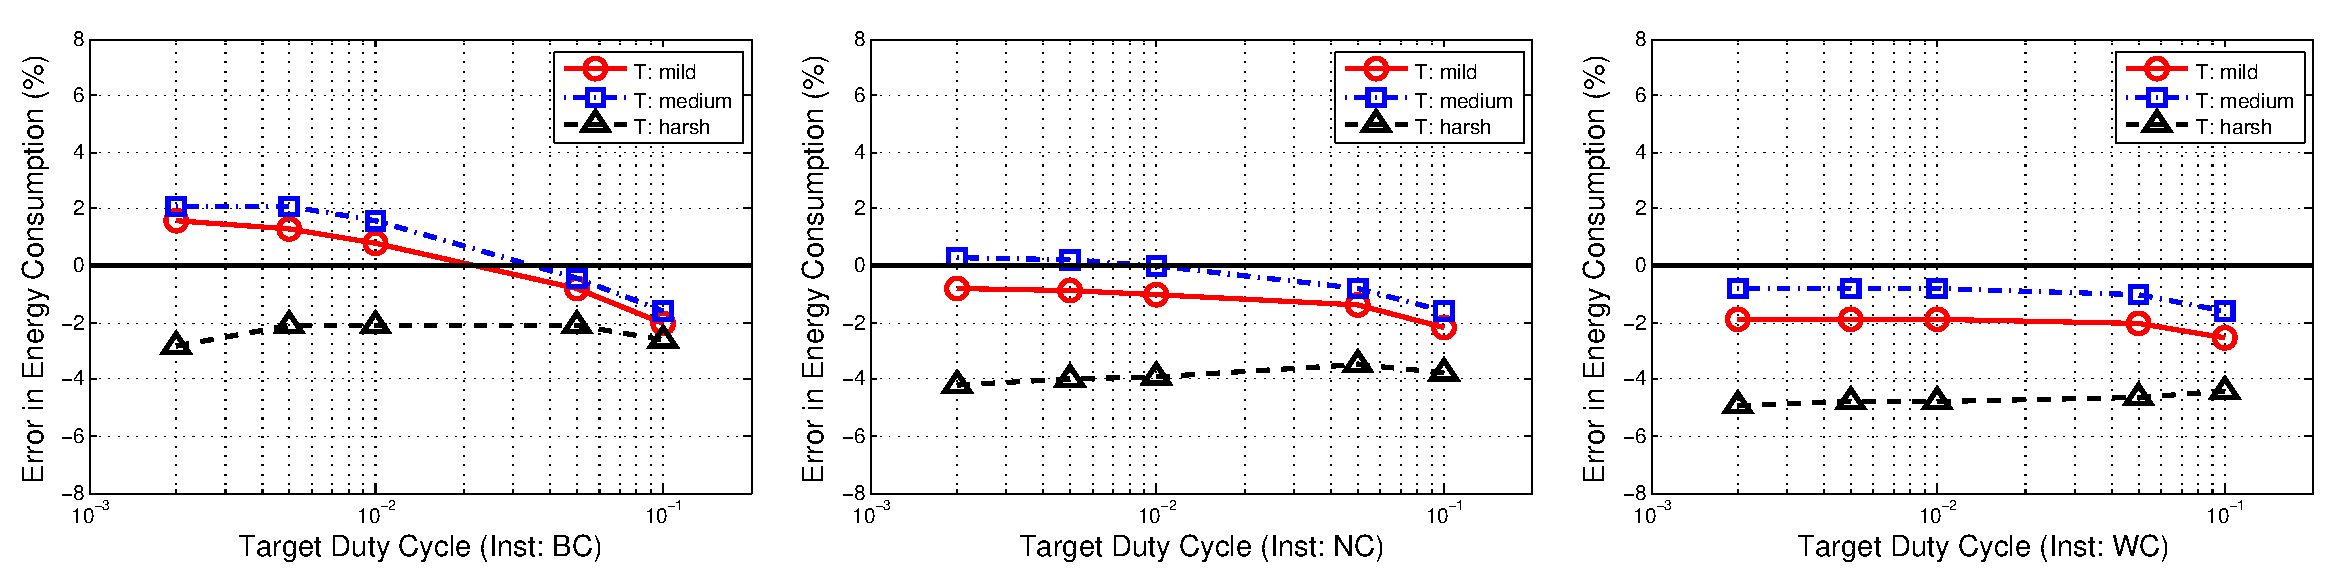
\includegraphics[width=1\textwidth]{figures/app1_nonoise.eps}
\caption{\label{fig:app1}App 1 results, no noise}
\end{figure*}

\begin{figure*}
\centering
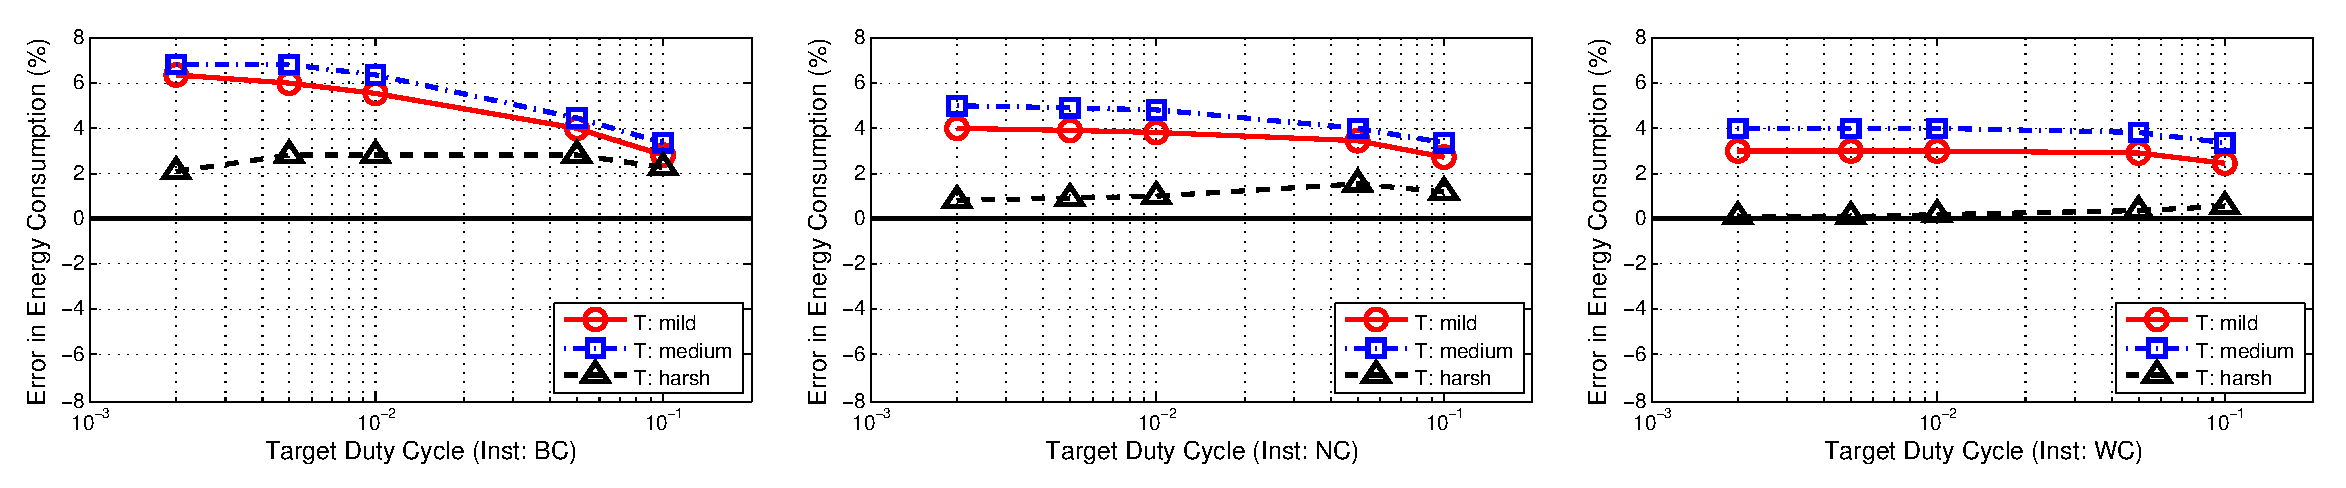
\includegraphics[width=1\textwidth]{figures/app1_guardband.eps}
\caption{\label{fig:app1}App 1 results, no noise}
\end{figure*}

\begin{figure}
\centering
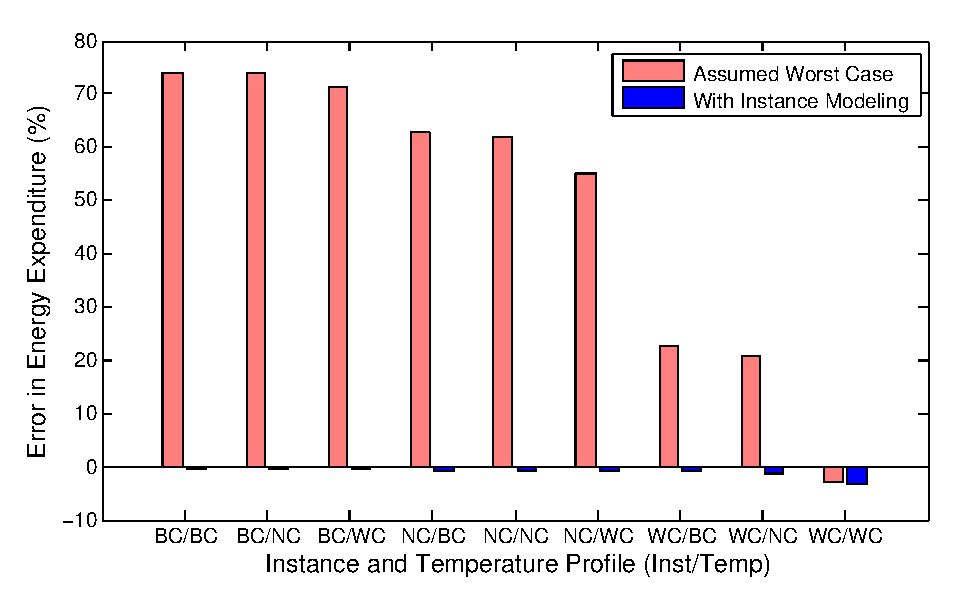
\includegraphics[width=1\columnwidth]{figures/app1_energycomp.eps}
\caption{\label{fig:app1}App 1 energy comparison}
\end{figure}

\begin{figure}
\centering
\includegraphics[width=1\columnwidth]{figures/app1_dutycycles.eps}
\caption{\label{fig:app1}App 1 dutycycle comparison}
\end{figure}

\begin{figure}
\centering
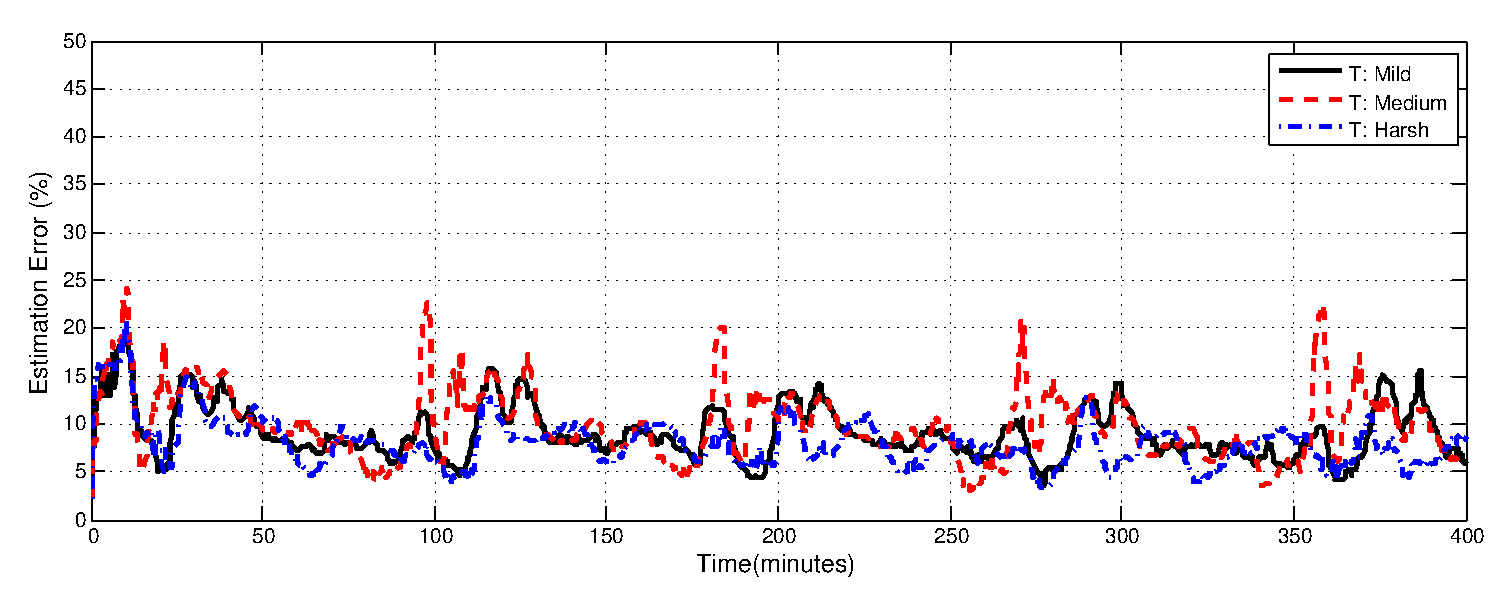
\includegraphics[width=1\columnwidth]{figures/localization_var.eps}
\caption{\label{fig:app1}App 1 dutycycle comparison}
\end{figure}



describe here the method of evaluation, introduce QEMU and VarEMU as tools for evaluation. Cite accuracy for varemu etc. 

\subsection{Multi-Sensor Applications}
Application 1: we have multiple sensors with various knobs fighting for resources with various utilities.

\subsection{Multi-Agent Applications}
Application 2: we have multiple agents and we seek to fuse data and make some inference like localization. Basically sensors + radio

\subsection{Digital Signal Processing Applications}
basically sensors + (tunable DSP stages) + radio
\input{sections/06_conclusion}

% use section* for acknowledgement
\section*{Acknowledgment}
The authors would like to thank...



%	REFERENCES		%
\bibliographystyle{IEEEtran}
\bibliography{bibliography}




% that's all folks
\end{document}


